\chapter{Results}


Analyzing the results obtained with the original parameters from 
the article by Parham and Michael 
($T' = 19.9 \ (\text{also called $T_1$ in the article}), \ T_1=23.2, \ T_2=0.07, \ \omega_1=0.67, \ \phi_1=1.53, \ R_1=85.9, \ R_2=0.98, 
\ \omega_2=0.65, \ \phi_2=1.99, \ A=-0.03, \ B=1.31, \ C=-4.4, \ b_1=0.04, \ 
b_2 = 0.09, \ T_{min}=14.5, \ \gamma= 1/120, \ R_L = 50, \ c_1=0.00554, \ 
c_2=-0.06737$ \cite{Parham2010}, \cite{OKUNEYE201772}), and using 
the previously estimated average population and an arbitrary value 
for the mosquito population, of 10000, assuming 1000 infected humans and 
5000 exposed mosquitoes at $t=0$, the modeling is as follows
\footnote{The development of the model with the original data can be found at 
https://github.com/RaphaLevy/Undergraduate\_Dissertation/blob/main/
\\modeling\_files/Original\_Parameters.ipynb.}: 

% Pra plotar duas imagens uma ao lado da outra, precisa corrigir a posição das legendas.

% \begin{figure}
% \hspace*{-1.5cm} % Adiciona espaço negativo para puxar a imagem para a esquerda
% \begin{minipage}{.45\textwidth}
%   \centering
%   \includegraphics[width=1.25\linewidth]{SIR_Dados_Originais_Parham_Michael.png}
%   \captionof{figure}{A figure}
%   \label{fig:test1}
% \end{minipage}%
% \hspace{1.5cm} % Adiciona espaço horizontal
% \begin{minipage}{.45\textwidth}
%   \centering
%   \includegraphics[width=1.3\linewidth]{SEI_Dados_Originais_Parham_Michael.png}
%   \captionof{figure}{Another figure} % Legenda à direita da segunda imagem
%   \label{fig:test2}
% \end{minipage}
% \end{figure}





\begin{figure}[!ht]
        \centering
        \hbox{\hspace{6em} 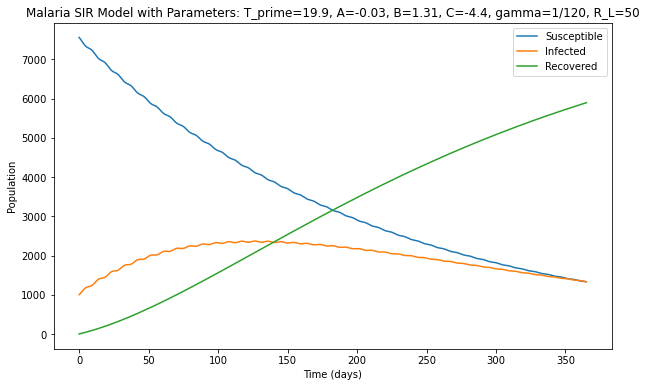
\includegraphics[scale=0.45] {THESIS-SIR_Dados_Originais_Parham_Michael_CORRECAO.png}}
        \caption{SIR with original parameters}
\end{figure} 
\begin{figure}[!ht]
        \centering
        \hbox{\hspace{6em} 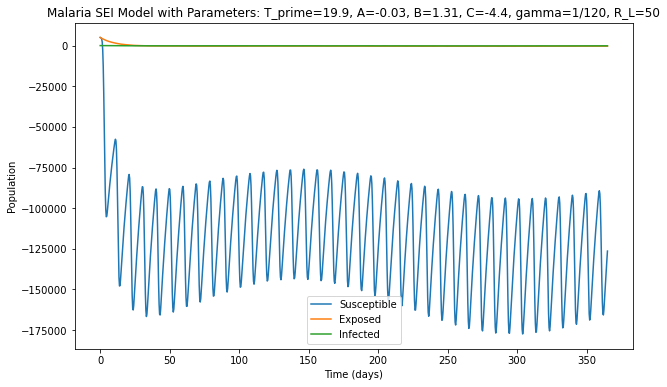
\includegraphics[scale=0.45] {THESIS-SEI_Dados_Originais_Parham_Michael_CORRECAO.png}}
        \caption{SEI with original parameters}
\end{figure} 
\newpage
With this initial modeling, 
a strong oscillation in the number 
of susceptible humans and mosquitoes, 
as well as infected humans, is noticeable. 
Furthermore, it is evident that with these 
parameters, the disease will not become endemic, 
as the number of infected humans tends to 0 
throughout the year, while the population of 
susceptible mosquitoes becomes negative, and the 
population of exposed and infected individuals also tends to 0. 
These effects were characterized by temperature and 
precipitation oscillating in very short periods of 
time, attributed to a high value of $\omega$ for both functions.
\\\\
Starting with only a single infected human and exposed mosquito, the 
oscilatting population isn't noticeable in the SIR plot, however the mosquito population 
still becomes negative.
\\\\
Now, the first necessary modification is to correct the temperature 
and precipitation to consider data from Manaus, as the original 
paper uses data from Tanzania. So, 
collecting climatological data from Manaus from \cite{ClimaMANAUS}, 
the average temperature and precipitation were estimated 
as 26.4 $^\circ C$ and 250.083 mm, respectively. 
With this data, the amplitude of seasonal variability, 
angular frequency, and phase lag of variability for 
both were defined to approximate the real values:
\\\\
\begin{adjustwidth}{-0.5cm}{}
\begin{center}
\renewcommand{\arraystretch}{1.5}
\begin{tabular}{|c | c|} 
 \hline
 \textbf{Parameter} & \textbf{Value}\\ 
 \hline
  $T_1$ & \makecell[l]{\rule{0pt}{3ex}26.4$^\circ C$\rule[-1.5ex]{0pt}{0pt}} \\
 \hline
 $T_2$ & \makecell[l]{\rule{0pt}{3ex}0.025\rule[-1.5ex]{0pt}{0pt}} \\
 \hline
 $\omega_1$ & \makecell[l]{\rule{0pt}{3ex}0.017 (months)$^{-1}$\rule[-1.5ex]{0pt}{0pt}} \\
 \hline
 $\phi_1$ & \makecell[l]{\rule{0pt}{3ex}-1.45\rule[-1.5ex]{0pt}{0pt}} \\
 \hline
 $R_1$ & \makecell[l]{\rule{0pt}{3ex}250.083 mm\rule[-1.5ex]{0pt}{0pt}} \\
 \hline
 $R_2$ & \makecell[l]{\rule{0pt}{3ex}0.565\rule[-1.5ex]{0pt}{0pt}} \\
 \hline
 $\omega_2$ & \makecell[l]{\rule{0pt}{3ex}0.02 (months)$^{-1}$\rule[-1.5ex]{0pt}{0pt}} \\
 \hline
 $\phi_2$ & \makecell[l]{\rule{0pt}{3ex}1.6\rule[-1.5ex]{0pt}{0pt}} \\
 \hline
\end{tabular}
\captionof{table}{Values for climatic parameters}
\end{center}
\end{adjustwidth}

\vspace{1cm}
The amplitude parameters ($T_2$ and $R_2$) and phase lag 
parameters ($\phi_1$ and $\phi_2$) are dimensionless. 
The temperature and precipitation throughout the year 
then evolve as follows
\footnote{The development of the model with the original data can be found at 
https://github.com/RaphaLevy/Undergraduate\_Dissertation/blob/main/
\\modeling\_files/Adapting\_T\_and\_R.ipynb.}:

% \begin{figure}
% \hspace*{-1.5cm} % Adiciona espaço negativo para puxar a imagem para a esquerda
% \begin{minipage}{.45\textwidth}
%   \centering
%   \includegraphics[width=1.2\linewidth]{Grafico_da_Temperatura.png}
%   \captionof{figure}{A figure}
%   \label{fig:test1}
% \end{minipage}%
% \hspace{1.5cm} % Adiciona espaço horizontal
% \begin{minipage}{.45\textwidth}
%   \centering
%   \includegraphics[width=1.2\linewidth]{Grafico_da_Precipitacao.png}
%   \captionof{figure}{Another figure} % Legenda à direita da segunda imagem
%   \label{fig:test2}
% \end{minipage}
% \end{figure}


\begin{figure}[!ht]
        \centering
        \hbox{\hspace{6.0em} 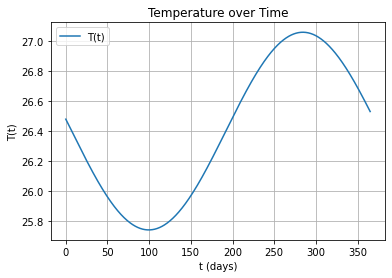
\includegraphics[scale=0.7] {THESIS-Grafico_da_Temperatura.png}}
        \caption{Temperature graph}
\end{figure} 
\begin{figure}[!ht]
        \centering
        \hbox{\hspace{6.5em} 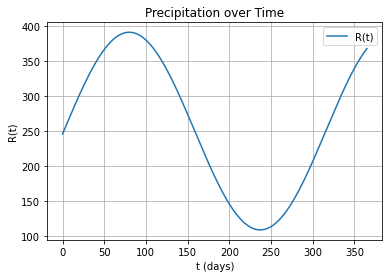
\includegraphics[scale=0.7] {THESIS-Grafico_da_Precipitacao.png}}
        \caption{Precipitation graph}
\end{figure} 
In order to ensure the correctness of the function 
with the parameters used, I calculated the temperature 
values for the months of October and May, which are the 
hottest and coldest months of the year with average 
temperatures of 27.6 $^\circ C$ and 25.8 $^\circ C$, respectively. 
Additionally, I calculated the precipitation values in March 
and August, which are the months with the highest and lowest 
precipitation, with 395 mm and 114 mm, respectively. 
The obtained average values were 27.06 $^\circ C$, 25.86 $^\circ C$, 
390.67 mm, and 112.89 mm. 
\\\\With the temperature and precipitation parameters ready for an 
initial analysis, the evolution of human and mosquito populations 
was verified.  
The results can be found in Appendices 1 and 2 
\footnote{The development of the graphs above can be found at 
https://github.com/RaphaLevy/Undergraduate\_Dissertation/blob/main/
\\modeling\_files/Adapting\_T\_and\_R.ipynb.}. 
\\\\
Notably, this result is still incorrect, as the mosquito population
still becomes negative over time. 
However, the daily oscillations
was indeed eliminated, due to the modifications made to $\omega_1$ and $\omega_2$.
Another parameter that should also be adapated in consideration for our new climatic
values was $R_L$, the rainfall limit beyond which breeding sites get flushed out and no 
immature stages survive. In the original paper, $R_L$ was defined as 50 mm, which is
too low for the high precipitation in the Amazon, which has a maximum of almost
400 mm in March. Because of this, I increased $R_L$ from 50 mm to 450 mm.
The results can be found in Appendices 3 and 4 
\footnote{The development of the graphs above can be found at 
https://github.com/RaphaLevy/Undergraduate\_Dissertation/blob/main/
\\modeling\_files/Adapting\_T\_and\_R.ipynb.}.
\\\\
Now, while the mosquito population in non-negative, it rapidly declines and
becomes extinct. That is due to the value of $\mu$, the mortality rate of mosquitoes,
given by $-\log(e^{(-1 / (AT^2 + BT + C))})$. For small values of 
$A$, $B$ and $C$, mostly $A$, $\mu$ becomes ``relatively'' large, and the mosquito
population goes extinct. To fix this, I altered these 3 parameters from the initial values 
of the arcticle, which had $\mu \approx 0.0027$, to $A=356.3, \ B=15$
and $C=-48.78$, which gave a $\mu$ of approximately $4.02133 \times 10^{-6}$, 
and so the mosquto population is nearly constant throughout the analysis.
The results, with $A, \ B$
and $C$ as above, can be found in Appendices 5 and 6 
\footnote{The development of the graphs above can be found at 
https://github.com/RaphaLevy/Undergraduate\_Dissertation/blob/main/
\\modeling\_files/Modifying\_Constant\_Parameters.ipynb.}.
\\\\
Now, it is possible to see that the mosquito population in fact remains nearly constant,
as there is close to no transference between compartments.
\\\\
To verify what else could be done to allow the 
transference of individuals between compartments,
given the differential equations of the SEI model and the 
parameters provided to achieve this goal, the value of $\mu$ becomes 
very close to 0, as seen above, while $l(\tau_M)$, a probability, becomes very 
close to 1. Therefore, $\dfrac{dE_M}{dt}$ also becomes very close to 0, 
causing the exposed function to be linear, while the mosquito population 
leaving the susceptible compartment almost simultaneously enters 
the infected compartment, causing mirrored oscillations of $S$ and $I$. 
To overcome this effect, it was necessary to modify the use of $b_1$ to 
only move mosquitoes from compartment $S$ to $E$, requiring the inclusion 
of a new parameter, $b_3$, to move mosquitoes from compartment $E$ to $I$. 
This rate is inversely related to the incubation period, so we define
\begin{gather*}
b_3 = \dfrac{T-T_{min}}{DD}
\end{gather*}
Moreover, the parameter $a(T)$ in the transition from 
exposed mosquitoes to infected was removed, as no new bites occur 
in this change from compartment $E$ to $I$.
\\\\
With these modifications, the differential equations of the SEI model were modified:
\begin{gather*}
\begin{cases}
\dfrac{dS_M}{dt} = b - ab_1\bigg(\dfrac{I_H}{N}\bigg)S_M - \mu S_M\\
\\
\dfrac{dE_M}{dt} = ab_1\bigg(\dfrac{I_H}{N}\bigg)S_M - \mu E_M - b_3E_Ml\\
\\
\dfrac{dI_M}{dt} = b_3E_Ml -\mu I_M\\
\end{cases}
\end{gather*}
\\\\
The results can be seen in Apendices 7 to 10, using $T'=19.9^\circ C$, as originally used,
and $T'=24.4^\circ C$, which is a value lower than the minimum temperature, close to $25.6^\circ C$.
Using $T'=19.9^\circ C$, the human population remains close to what could be seen in Appendix 5,
while the mosquito population is now oscillating, with the number of exposed 
mosquitoes decreasing to values near 0, while the infected population increases.
With $T'=24.4^\circ C$, the SEI plot is very similar, however the increase 
of the infected population is less noticeable.
In the case of the human population, it can be seen that the disease begins 
at a later time, and the maximum number of infected individuals is lower than
what was seen before
\footnote{The development of the graphs above can be found at 
https://github.com/RaphaLevy/Undergraduate\_Dissertation/blob/main/
\\modeling\_files/SEI\_Exposed\_to\_Infected.ipynb.}.
\\\\
Another necessary modification was to disassociate $l$, the probability of mosquito 
survival during the sporozoite cycle, from the infection rate of exposed individuals $b_3$.
\begin{gather*}
        \begin{cases}
        \dfrac{dS_M}{dt} = b - ab_1\bigg(\dfrac{I_H}{N}\bigg)S_M - \mu S_M\\
        \\
        \dfrac{dE_M}{dt} = ab_1\bigg(\dfrac{I_H}{N}\bigg)S_M - \mu E_M - b_3E_M -lE_M\\
        \\
        \dfrac{dI_M}{dt} = b_3E_M -\mu I_M\\
        \end{cases}
        \end{gather*}
With this alteration, it was noted that both populations didn't reach an equilibrium
in the first year of analysis, so extending it to 5 years, the results were as seen in Appendices 11 to 14 
\footnote{The development of the graphs above can be found at 
https://github.com/RaphaLevy/Undergraduate\_Dissertation/blob/main/
\\modeling\_files/SEI\_Exposed\_to\_Infected.ipynb.}. 
\\\\
With the SIR/SEI model now properly corrected, it was possible 
to proceed with the analyses of deforestation application. 
To do so, I began by calculating the $\mathcal{R}_0$ for both SIR and SEI, 
as well as for the coupled model, using the formulation from 
P. van den Driessche \cite{VANDENDRIESSCHE200229} as a reference:
\\\\
Firstly, we define $X_s$ as the set of all disease-free states, 
$$X_s=\{x \geq 0|x_i=0, i=1,\ldots,m\},$$
where $X=(x_1,\ldots, x_n)^T$, such that $x_i\geq 0$ represents the number 
of individuals in each compartment, and we assume each function to be 
continuously differentiable at least twice in each variable ($C^2$).
\\\\
Now, we rearrange the equations so that the first $m$ equations 
contain the infected individuals. Let ${\mathcal F}_i(x)$ be the 
rate of appearance of new infections in compartment $i$, 
${\mathcal V}_i^+(x)$ be the rate of individuals entering 
compartment $i$ by other means, and ${\mathcal V}_i^-(x)$ 
be the rate of individuals leaving compartment $i$. The disease 
transmission model consists of non-negative initial conditions 
together with the following system of equations:
$$\dot{x}=f_i(x)={\mathcal F}_i(x)-{\mathcal V}_i(x), i=1,\ldots, n,$$
where ${\mathcal V}_i (x) = {\mathcal V}_i^{-}(x) - {\mathcal V}_i^+(x)$. 
We also define 
$F=\left[\frac{\partial {\mathcal F}_i (x_0)}{\partial x_j}\right]$ 
and $V=\left[\frac{\partial {\mathcal V}_i (x_0) }{\partial x_j}\right]$, 
where $x_0$ is a Disease-Free Equilibrium (DFE), and $1\leq i,j \leq m$.
\\\\
This is equivalent to the Jacobian of these two matrices, 
after substituting $x_0$, i.e., $S=1$. $\mathcal{R}_0$ will be given 
by $\rho(FV^{-1})$, in other words, it will be the spectral radius 
of the matrix $FV^{-1}$. With the necessary definitions, we can 
calculate the $\mathcal{R}_0$ for both models as follows:
\begin{itemize}
\item \textbf{SIR:}
In this case, $m=1$, and our compartments will be arranged as $[I_H, S_H, R_H]$. Since $\mathcal{R}_0$ is calculated with normalized values, we will multiply the necessary equations by $N$ to remove the denominator. Specifically, for the SIR case, as $R_H$ is not used in any of the equations, we can express it solely in terms of $S$ and $I$. Therefore:
$$ {\mathcal F}_i(x): \text{ rate of appearance of new infected individuals in compartment } i $$
$$ {\mathcal F} =\begin{bmatrix}
a  b_2  I_M  S_H \\
\end{bmatrix} $$
Additionally, we have
$$ {\mathcal V}_i(x)^-: \text{ rate of leaving compartment } i $$
$$ {\mathcal V}_i(x)^+: \text{ rate of entering compartment } i $$
Thus:
$$
{\mathcal V^-} = \begin{bmatrix}
\gamma I_H\\
\end{bmatrix}
$$
$$
{\mathcal V^+} = \begin{bmatrix}
0\\
\end{bmatrix}
$$
$${\mathcal V}_i (x) = {\mathcal V}_i(x)^{-} - {\mathcal V}_i(x)^+$$
Therefore,
$$
{\mathcal V} =
\begin{bmatrix}
\gamma I_H\\
\end{bmatrix}
$$
\\
Hence
$$ F = \dfrac{\partial{\mathcal F}}{\partial I_M} =\begin{bmatrix}
a  b_2  S_H \\
\end{bmatrix} $$
$$ V = \dfrac{\partial{\mathcal V}}{\partial I_H} =\begin{bmatrix}
\gamma \\
\end{bmatrix} $$
\\At the equilibrium, $[S_H^*, I_H^*] = [1,0]$, so $F=[a  b_2], \ V = [\gamma]$ and $\mathcal{R}_0 = \Big | \dfrac{ab_2}{\gamma}\Big | $.

\item \textbf{SEI:}
In this case, $m=2$, and our compartments will be arranged as $[E_M, I_M, S_M]$. Again, we multiply the necessary equations by $N$ to remove the denominator. Therefore:
$$ {\mathcal F} =\begin{bmatrix}
a b_1 I_H S_M\\
0\\
\end{bmatrix} $$
$$
{\mathcal V^-} = \begin{bmatrix}
E_M (\mu + b_3 + l)\\
\mu I_M
\end{bmatrix}
$$
$$
{\mathcal V^+} = \begin{bmatrix}
0\\
b_3 E_M\\
\end{bmatrix}
$$
$${\mathcal V}_i (x) = {\mathcal V}_i(x)^{-} - {\mathcal V}_i(x)^+$$
Thus,
$$
{\mathcal V} =
\begin{bmatrix}
E_M (\mu + b_3 + l)\\
\mu I_M - b_3 E_M\\
\end{bmatrix}
$$
\\
Hence
$$ F = \dfrac{\partial{\mathcal F}}{\partial E_M, I_H} =\begin{bmatrix}
\dfrac{\partial ab_1 I_H S_M}{\partial E_M} & \dfrac{\partial ab_1 I_H S_M}{\partial I_H}\\
\dfrac{\partial 0}{\partial E_M} & \dfrac{\partial 0}{\partial I_H}\\
\end{bmatrix} = 
\begin{bmatrix}
0 & ab_1 S_M\\
0 & 0\\
\end{bmatrix}$$
$$ V = \dfrac{\partial{\mathcal V}}{\partial E_M, I_M} =\begin{bmatrix}
\dfrac{\partial E_M (\mu + b_3 + l)}{\partial E_M} & \dfrac{\partial E_M (\mu + b_3 + l)}{\partial I_M}\\
\dfrac{\partial \mu I_M - b_3 E_M}{\partial E_M} & \dfrac{\partial \mu I_M - b_3 E_M}{\partial I_M}\\
\end{bmatrix} = 
\begin{bmatrix}
\mu+b_3+l & 0\\
- b_3 & \mu\\
\end{bmatrix}$$
\\At the equilibrium, $[S_M^*, E_M^*, I_M^*] = [1,0,0]$, so $$F=\begin{bmatrix}
0 & ab_1\\
0 & 0\\
\end{bmatrix},$$
$$V = \begin{bmatrix}
\mu+b_3+l & 0\\
- b_3 & \mu\\
\end{bmatrix}$$ and $\mathcal{R}_0 = \Big | \dfrac{ab_1b_3}{(b_3+l+\mu)\mu}\Big | $.

\item \textbf{SIR/SEI:}
In this case, $m=3$, and our compartments will be arranged as $[I_H, E_M, I_M, S_H, S_M]$. Once again, we multiply the necessary equations by $N$ to remove the denominator. Therefore:
$$ {\mathcal F} =\begin{bmatrix}
a  b_2  I_M  S_H \\
a b_1 I_H S_M\\
0\\
\end{bmatrix} $$
$$
{\mathcal V^-} = \begin{bmatrix}
\gamma I_H\\
E_M (\mu + b_3 + l)\\
\mu I_M
\end{bmatrix}
$$
$$
{\mathcal V^+} = \begin{bmatrix}
0\\
0\\
b_3 E_M \\
\end{bmatrix}
$$
$${\mathcal V}_i (x) = {\mathcal V}_i(x)^{-} - {\mathcal V}_i(x)^+$$
Thus,
$$
{\mathcal V} =
\begin{bmatrix}
I_H \gamma \\
E_M (\mu + b_3 + l)\\
\mu I_M - b_3 E_M\\
\end{bmatrix}
$$
\\
Hence
$$ F = \dfrac{\partial{\mathcal F}}{\partial I_H, E_M, I_M} =\begin{bmatrix}
\dfrac{\partial ab_2 I_M S_H}{\partial I_H} & \dfrac{\partial ab_2 I_M S_H}{\partial E_M} & \dfrac{\partial ab_2 I_M S_H}{\partial I_M}\\
\dfrac{\partial ab_1 I_H S_M}{\partial I_H} & \dfrac{\partial ab_1 I_H S_M}{\partial E_M} & \dfrac{\partial ab_1 I_H S_M}{\partial I_M}\\
\dfrac{\partial 0}{\partial I_H} & \dfrac{\partial 0}{\partial E_M} & \dfrac{\partial 0}{\partial I_M}\\
\end{bmatrix} = 
\begin{bmatrix}
0 & 0 & ab_2 S_H\\
ab_1 S_M & 0 & 0\\
0 & 0 & 0
\end{bmatrix}$$
$$ V = \dfrac{\partial{\mathcal V}}{\partial I_H, E_M, I_M} =\begin{bmatrix}
\dfrac{\partial \gamma I_H}{\partial I_H} & \dfrac{\partial \gamma I_H}{\partial E_M} & \dfrac{\partial \gamma I_H}{\partial I_M}\\
\dfrac{\partial E_M (\mu + b_3 + l)}{\partial I_H} & \dfrac{\partial E_M (\mu + b_3 + l)}{\partial E_M} & \dfrac{\partial E_M (\mu + b_3 + l)}{\partial I_M}\\
\dfrac{\partial \mu I_M - b_3 E_M}{\partial I_H} & \dfrac{\partial \mu I_M - b_3 E_M}{\partial E_M} & \dfrac{\partial \mu I_M - b_3 E_M}{\partial I_M}\\
\end{bmatrix} = 
$$
$$
\begin{bmatrix}
\gamma & 0 & 0\\
0 & b_3+l+\mu & 0\\
0 & -b_3 & \mu
\end{bmatrix}$$
\\At the equilibrium, $[S_H^*, S_M^*, I_H^*, E_M^*, I_M^*] = [1,1,0,0,0]$, so $$F=\begin{bmatrix}
0 & 0 & ab_2\\
ab_1 & 0 & 0\\
0 & 0 & 0
\end{bmatrix},$$
$$V = \begin{bmatrix}
\gamma & 0 & 0\\
0 & b_3+l+\mu & 0\\
0 & -b_3 & \mu
\end{bmatrix}$$ 
and $\mathcal{R}_0 = \Big | \sqrt{\dfrac{a^2 b_1 b_2 b_3}{(b_3 + l + \mu)\gamma \mu}}\Big | = 
\sqrt{\mathcal{R}_{0 SIR} \times \mathcal{R}_{0 SEI}}$. 
\end{itemize}
We can verify that $\mathcal{R}_0$ is indeed dimensionless: 
$a, \ b_3, \ l, \ \mu$, and $\gamma$ are functions with units 
of 1/day, while $b_1$ and $b_2$ are dimensionless. Therefore, 
$\mathcal{R}_0$ for the SIR model has dimensions of (1/day)/(1/day), 
$\mathcal{R}_0$ for the SEI model has dimensions of (1/day$^2$)/(1/day$^2$), 
and the coupled model has dimensions of (1/day$^3$)/(1/day$^3$).
\\\\
Before continuing with the modeling, it was decided to analyze the evolution
of the rates as a function of temperature and precipitation, instead of time,
to see their behavior as $T$ and $R$ vary. In this case, $T'$ was used 
with value $25.6^{\circ}C$, in order to approximate
$\mathcal{R}_0$ to 0.5, which will be used later in the dissertation. 
The results can be found starting on
Appendix 15 
\footnote{The development of the graphs above can be found at 
https://github.com/RaphaLevy/Undergraduate\_Dissertation/blob/main/
\\modeling\_files/Plotting\_Rates.ipynb.}.
\\\\
Now, having the formula for $\mathcal{R}_0$ for the coupled model,
the model was executed starting with $E_{M0}=1$ and $I_{M0}=1$ and with
$E_{M0}=50000$ and $I_{M0}=1000$
\footnote{These results can be found respectively at
https://github.com/RaphaLevy/Undergraduate\_Dissertation/blob/main/
\\modeling\_files/Plotting\_with\_R0.ipynb and
https://github.com/RaphaLevy/Undergraduate\_Dissertation/blob/main/
\\modeling\_files/Plotting\_with\_R0\_2.ipynb.}. With the parameters used
in Appendices 13 and 14, $\mathcal{R}_0$ was calculated to be 5.99, which
means the disease becomes endemic, as it's value is greater than 1. Using $T'=25.6^{\circ}C$
and $A=12.5$, the results were seen as below:
\newpage
\begin{figure}[!ht]
        \centering
        \hbox{\hspace{2.8em} 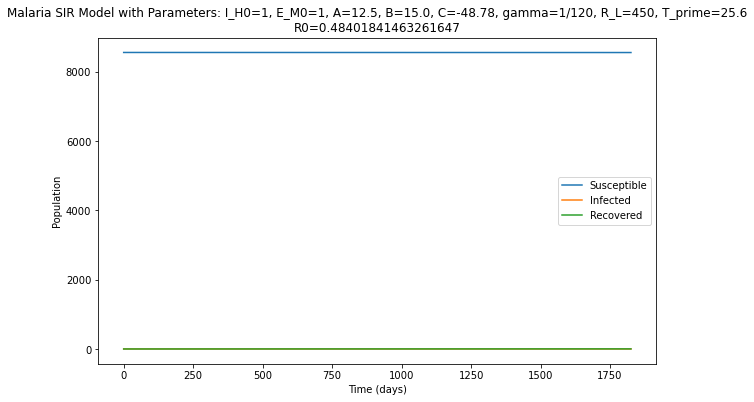
\includegraphics[scale=0.5] {THESIS-SIR_Initial_EI_1_R0_leq_1.png}}
        \caption{SIR with $\mathcal{R}_0 <1$, starting with $E_{M0}$ and $I_{M0}=1$}
\end{figure} 
\begin{figure}[!ht]
        \centering
        \hbox{\hspace{2.8em} 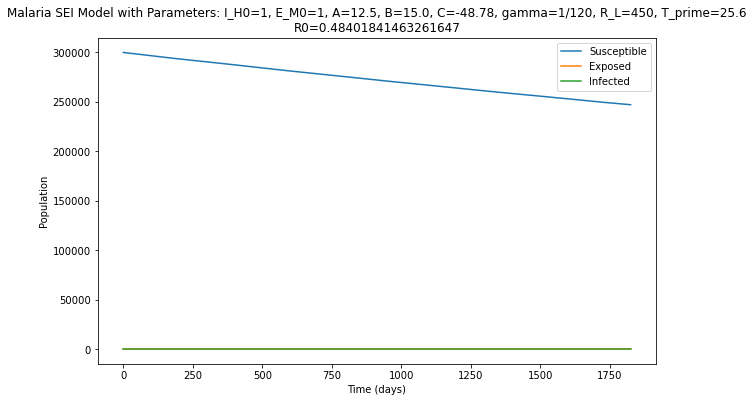
\includegraphics[scale=0.5] {THESIS-SEI_Initial_EI_1_R0_leq_1.png}}
        \caption{SEI with $\mathcal{R}_0 <1$, starting with $E_{M0}$ and $I_{M0}=1$}
\end{figure}
\newpage
\begin{figure}[!ht]
        \centering
        \hbox{\hspace{2.5em} 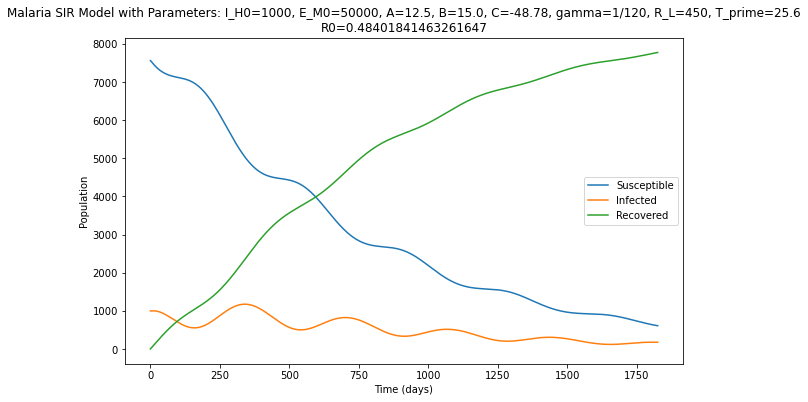
\includegraphics[scale=0.5] {THESIS-SIR_Initial_EI_geq_1_R0_leq_1.png}}
        \caption{SIR with $\mathcal{R}_0 <1$, starting with $E_{M0}$ and $I_{M0}>1$}
\end{figure} 
\begin{figure}[!ht]
        \centering
        \hbox{\hspace{2.5em} 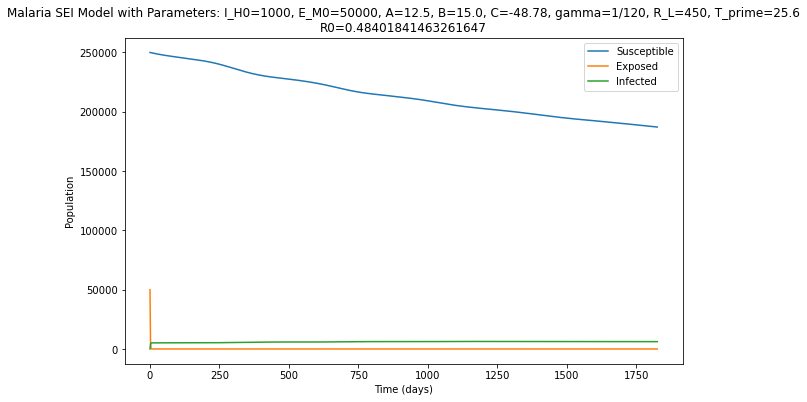
\includegraphics[scale=0.5] {THESIS-SEI_Initial_EI_geq_1_R0_leq_1.png}}
        \caption{SEI with $\mathcal{R}_0 <1$, starting with $E_{M0}$ and $I_{M0}>1$}
\end{figure}
With this, as expected, we can see that the disease dies out, specifically 
the susceptible mosquito population. This would be due to the mortality rate
being higher than the birth rate.
\\\\Having the model ready, it was possible to proceed with the analysis of
the impacts of deforestation. To do that, it was decided to include a multypling
factor $k$ for the infection rates of both models, substituting $ab_1$ and
$ab_2$ by $kab_1$ and $kab_2$, respectively. This factor will be used to represent 
the increasing contact between human and mosquito populations due to the
the approximation caused by this environental change. With that in mind, 
we are interested to see how the disease behaves as $k$ increases, therefore
as the contact between the populations increases.
\\\\
To do this, it was also decided that, instead of using the estimated population 
of the rural region of Manaus of 8558, use the population estimated via interpolation 
for 2004, and include a birth and mortality rate for the human population, $\mu_H$. 
With the previously obtained values for the human population 
between 2004 and 2009, the annual birth rate was 
estimated to be 206.8 births per year. Therefore, this corresponds 
to approximately 0.56657 births per day and 0.00007 births per day 
per person, given that the average rural population in Manaus is 
approximately 8078.5 people between 2004 and 2008. Therefore, using $\mu_h = 0.00007$ 
and $k$, the final model is given by:
\begin{gather*}
        \begin{cases}
        \dfrac{dS_H}{dt} = \mu_HN-akb_2\bigg(\dfrac{I_M}{N}\bigg)S_H - \mu_HS_H\\
        \\
        \dfrac{dI_H}{dt} = akb_2\bigg(\dfrac{I_M}{N}\bigg)S_H-\gamma I_H - \mu_HI_H\\
        \\
        \dfrac{dR_H}{dt} = \gamma I_H - \mu_HR_H\\
        \\
        \dfrac{dS_M}{dt} = b - akb_1\bigg(\dfrac{I_H}{N}\bigg)S_M - \mu S_M\\
        \\
        \dfrac{dE_M}{dt} = akb_1\bigg(\dfrac{I_H}{N}\bigg)S_M - \mu E_M - b_3E_M -lE_M\\
        \\
        \dfrac{dI_M}{dt} = b_3E_M -\mu I_M\\
        \end{cases}
        \end{gather*}
Where $\mathcal{R}_0$ for SIR is given by $\Big | \dfrac{akb_2}{\gamma + \mu_H}\Big | $,
for SEI is given by $\Big | \dfrac{akb_1b_3}{(b_3 + l + \mu)\mu}\Big | $
and for the coupled model is given by $\Big | \sqrt{\dfrac{a^2k^2b_1b_2b_3}{(b_3+l+\mu)(\gamma+\mu_H)\mu}}\Big | $.
It can be immediately seen that $k$ will have a linear impact on
$\mathcal{R}_0$.
\\\\
The results using $k=1.5, \ 2, \ 2.5, \ 5$ and $10$ can be found in Appendices 
27 to 36, while plots for each population for multiple values 
of $k$ can be found in Appendices 37 to 42. The results with $k=1$ 
is seen in Figures 5 and 6 \footnote{These results can be found respectively at
https://github.com/RaphaLevy/Undergraduate\_Dissertation/blob/main/
\\modeling\_files/Plotting\_with\_k.ipynb.}.
\\\\
It can be seen that, even starting with a single infected 
human and exposed mosquito,
the disease will eventually become endemic. For $k$ ranging between 1 and 2,
$\mathcal{R}_0$ is less than 1, so the disease will die out. However, for $k=2.5$, 
$\mathcal{R}_0>1$, and it is possible to see, even if only at the end of the analysis, that the disease 
starts to become endemic, as the human population of infected and recovered 
have a slight increase by $t=1500$. For the mosquito population, this 
behavior is less evident.
\\\\
For $k=5$ and $k=10$, the disease is already endemic, as it is possible to see
how it evolves, and that the population will eventually be nearly completely 
recovered from malaria in the case of the human population. Comparing the results 
of SIR between $k=5$ and $k=10$, the most notable difference is that, the larger 
the value of $k$, consequently the larger the value of $\mathcal{R}_0$, 
the faster the disease becomes endemic. For the SEI model, the difference 
is that the population stabilizes at different ranges. For $k$ up to 2.5, 
it appears that the disease doesn't become endemic, atleast in the first 5 years 
of the analysis. This may also be due to the large value of $M$, meaning the the exposed and 
infected mosquito populations are very small relatively to the susceptible population.
\\\\
For $k=5$ or 10, the sueceptible population rapidly decreases at 
a certain point in time, and the infected has a slight increase. In 5 years,
the population seems to become stable, however it would be possible to confirm 
if that's the case by increasing the maximum time of analysis.
\\\\
Now, we can see that we may double the infection rates, and the disease still 
won't become endemic. In the image below, it is shown how $\mathcal{R}_0$ 
increases as $k$ increases:
\begin{figure}[!ht]
        \centering
        \hbox{\hspace{2.5em} 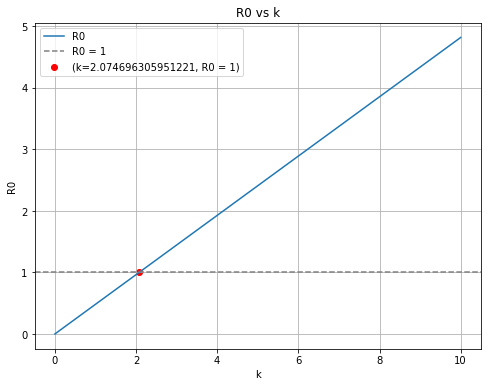
\includegraphics[scale=0.75] {THESIS-R0_vs_k.png}}
        \caption{$\mathcal{R}_0$ given in function of $k$}
\end{figure}
\newpage
So, using the parameters from Figures 7 and 8, we can see how the disease 
will only become endemic when $k>2.075$. Using this results, we can see that
deforestation does indeed cause a significant impact on the disease,
as increasing the biting rate in up to 5 to 10 times, starting with a single 
infected/exposed individual will lead the disease to infect a large portion 
of the human population, nearly $40\%$, before decreasing into a stable 
recovered population.
\\\\
In fact, we may analyze how the equilibriums of $S_H$ and $I_H$ are 
affected in function of $k$:
\begin{figure}[!ht]
        \centering
        \hbox{\hspace{5.0em} 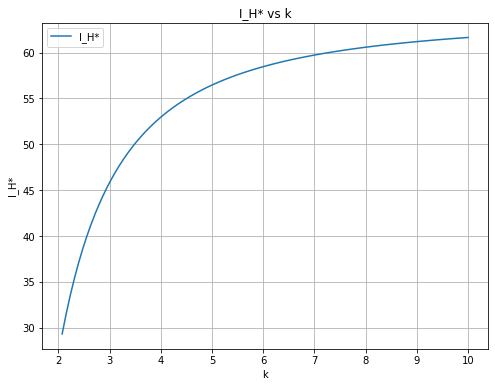
\includegraphics[scale=0.6] {THESIS-Equilibrium_IH_vs_k.png}}
        \caption{$I_H^*$ given in function of $k$}
\end{figure}
\begin{figure}[!ht]
        \centering
        \hbox{\hspace{5.0em} 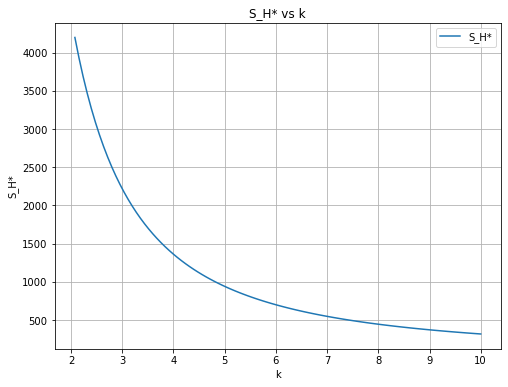
\includegraphics[scale=0.6] {THESIS-Equilibrium_SH_vs_k.png}}
        \caption{$S_H^*$ given in function of $k$}
\end{figure}
\\\\
By starting the plots for $k$ which makes $\mathcal{R}_0 = 1$ and for $t=1825$, 
as we want the final equilibrium, 
it is possible to see that the endemic equilibrium of infected 
humans approaches to a little over 60 as $k$ increases to 10. 
In fact, when $k=10$, $I_H^* \approx 61.64$. Analyzing the 
susceptible population, it decreases to values under 500, 
$S_H^* \approx 317$ when $k=10$ \footnote{These results can be found respectively at
https://github.com/RaphaLevy/Undergraduate\_Dissertation/blob/main/
\\modeling\_files/Plotting\_Equilibriums.ipynb.}.
\\\\ 
Iniciando o plot a partir de $k$ que deixa $\mathcal{R}_0 = 1$, é possível ver que
o equilíbrio endêmico da população humana se aproxima de 64 conforme $k$ se aproxima de 10.
Mais especificamente, quando $k=10$, $I_H^* \approx 63.49$ \footnote{A elaboração 
dos gráficos em função de $k$ podem ser encontrados em https://github.com/RaphaLevy/TCC/blob/main/Modelagem\_com\_Dinamica\_Pop/Plota\_Equilibrio\_e\_R0.ipynb. 
O cálculo dos equilíbrios pode ser encontrado em
https://github.com/RaphaLevy/TCC/blob/main/Modelagem\_com\_Dinamica\_Pop/R0\_com\_Dinamicas\_Demograficas.ipynb}.
Analisando o equilíbrio de suscetíveis conforme $k$ aumenta, é possível 
ver o equilíbrio decaindo rapidamente
de $N$ quando $k=0$ para aproximadamente 5000 indivíduos quando $k=1$. Analisando 
nos valores de $k$ tais que $\mathcal{R}_0 \geq 1$:
% \begin{figure}[!ht]
%         \centering
%         \hbox{\hspace{4.2em} \includegraphics[scale=0.7] {Plot_S_H_vs_k.png}}
%         \caption{$S_H^*$ em função de $k$}
% \end{figure} 
\newpage
Nesse caso, a população de suscetíveis tende a aproximadamente 95 conforme 
$k$ se aproxima de 10. Tendo calculado os equilíbrios de $S_H$ e $I_H$,
foi possível fazer uma análise de estabilidade global. Como estamos interessados
em analisar o equilíbrio endêmico, utilizei $k=10$:
\begin{figure}[!ht]
        \centering
        \hbox{\hspace{2.2em} \includegraphics[scale=0.7] {Equilibrio_SH_IH_k_10.png}}
        \caption{Equilíbrio global $S_H^* \times I_H^*$ para $k=10$}
\end{figure}
\\\\
Nesse caso, foram feitas 6 análises, a primeira utilizando os
valores iniciais de $S_H$ e $I_H$ como sendo 7716 e 1, e as demais aumentando $I_H$ 
em 1000 e diminuindo $S_H$ em 1000 indivíduos. Nesse caso, é possível
ver as populações de suscetíveis e infectados com um equilíbrio final de
aproximadamente 8 e 70 pessoas, respectivamente. Com isso,
poderíamos comparar o resultado obtido com o cálculo do equilíbrio endêmico de Adda e Bichara
\cite{adda2011global}, onde
\begin{gather*}
        S_H^* = \dfrac{1}{\mathcal{R}_0} \\
        I_H^* = \dfrac{\mu_H}{\mu_H+\gamma}(1-\dfrac{1}{\mathcal{R}_0})
\end{gather*}       
Através desse cálculo, a população de suscetíveis e infectados no equilíbrio 
foi de aproximadamente 1601 e 51, respectivamente. Notavelmente, esses valores 
estão destoantes dos 
obtidos através do cálculo numérico. Contudo, é necessário considerar a principal diferença entre as equações
propostas para $S$ e $I$ nesse Trabalho e no artigo de Adda e Bichara, que é o uso de
$I_M$ na taxa de infecção $\beta$, dada a dinâmica do modelo 
acoplado de SIR e SEI nesse caso, que não está sendo considerada no trabalho
de Adda e Bichara.